% ------------------
\mysec{Strahlensatz}
% ------------------
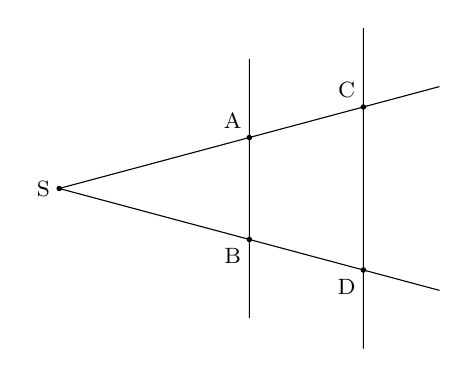
\begin{tikzpicture}[rotate=-15]
  \draw (0.0, 0) -- (5.0000, 0.0000); % unterer Strahl
  \draw (0.0, 0) -- (4.3301, 2.5000); % oberer Strahl
  \draw (1.90620,  2.21590) -- (2.75882, -0.96593); % erste Parallele
  \draw (3.20530,  2.96590) -- (4.25882, -0.96593); % zweite Parallele
  \fill (0.000, 0.000) circle (1pt); % S
  \fill (2.500, 0.000) circle (1pt); % B
  \fill (4.000, 0.000) circle (1pt); % D
  \fill (3.464, 2.000) circle (1pt); % C
  \fill (2.165, 1.250) circle (1pt); % A
  \node[shift=(180:2mm)] at (0.000, 0.000) {{\footnotesize S}};
  \node[shift=(135:3mm)] at (2.165, 1.250) {{\footnotesize A}};
  \node[shift=(225:3mm)] at (2.500, 0.000) {{\footnotesize B}};
  \node[shift=(135:3mm)] at (3.464, 2.000) {{\footnotesize C}};
  \node[shift=(225:3mm)] at (4.000, 0.000) {{\footnotesize D}};
\end{tikzpicture}\bigskip
\formrow{\frac{\;\overline{SA}\;}{\overline{SC}}=\frac{\;\overline{SB}\;}{\overline{SD}}=\frac{\;\overline{AB}\;}{\overline{CD}}}
\formrow{\frac{\;\overline{AC}\;}{\overline{SC}}=\frac{\;\overline{BD}\;}{\overline{SD}}}
\formrow{\frac{\;\overline{SA}\;}{\overline{AC}}=\frac{\;\overline{SB}\;}{\overline{BD}}}

